\begin{frame}
    \frametitle{資料}
    
    \begin{itemize}
        \item 墨西哥嫖妓交易資料
        \item 解釋變數:ln(交易價格)
        \item 被解釋變數: BAR、STREET、SCHOOL、AGE、RICH、ALCOHOL、ATTRACTIVE
    \end{itemize}
\end{frame}

\begin{frame}
    \frametitle{有無質性?}

    先從直覺上,漂亮的性工作者,價錢或許得以持續開很高,而長相較為不佳者,價錢的變動或許較高。
    \begin{figure}
        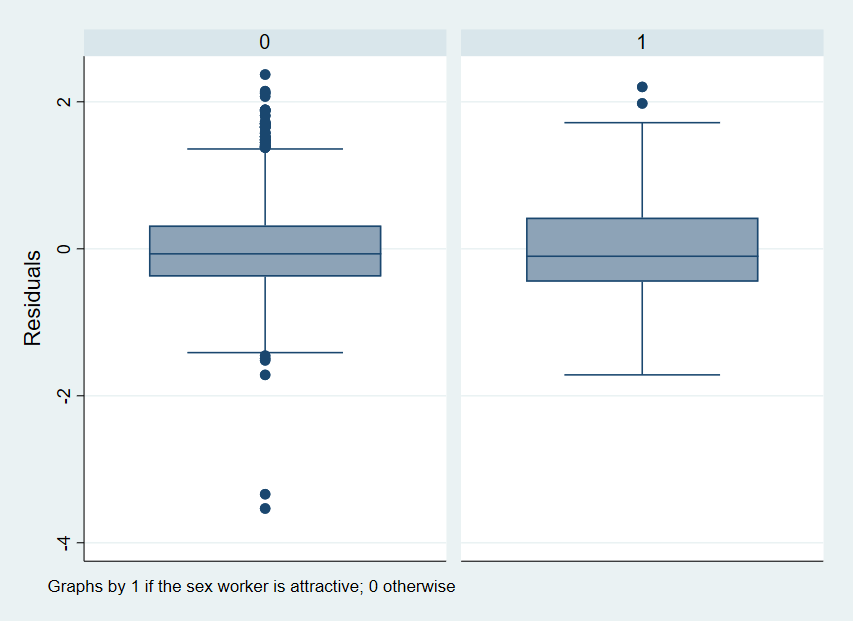
\includegraphics[width=0.8\textwidth]{../Results/boxplot_attractive_res.png}
    \end{figure}
\end{frame}

\begin{frame}[fragile]
    \frametitle{針對 attractive 測試異質變異數 --- NR2 test}
    作法一、土法煉鋼
    \begin{enumerate}
        \item 拿殘差項平方對 ATTRACTIVE 回歸
        \item 算出 $nr2=N\times R^2$
        \item 自由度 = 1
        \item 算出1\% 顯著水準下的臨界值 \texttt{invchi2tail(1, 0.01)}
        \item p-value :\texttt{chi2tail(1, nr2)}
    \end{enumerate}

    \begin{lstlisting}
predict res_a, res
gen res_a2=res_a^2

eststo het_nr2 : reg res_a2 attractive
scalar nr2=e(N)*e(r2)

di "NR2 value:" nr2
di "Critical value: " invchi2tail(1, 0.01)
di "P value :" chi2tail(1, nr2) \end{lstlisting}

\end{frame}
\begin{frame}[fragile]
    作法二、內建指令進行 NR2 test

    \begin{lstlisting}
est restore est_a
estat hettest attractive, iid \end{lstlisting}

    \vfill
    \begin{alertblock}{注意!}
        在土法煉鋼算 NR2 test 時,要用的是殘差對變數的回歸。
        而在使用內建指令時,不用特別進行殘差項的回歸,而是要將原本的回歸變成目前的回歸(也就是要 \texttt{est restore est\_a})。
    \end{alertblock}
\end{frame}

\begin{frame}[fragile]
    \frametitle{針對 attractive 測試異質變異數 --- NR2 test}
    作法一、土法煉鋼
    \begin{enumerate}
        \item 拿殘差項平方對 ATTRACTIVE 回歸
        \item (聯合)檢定殘差項回歸的係數
    \end{enumerate}

    \begin{lstlisting}
predict res_a, res
gen res_a2=res_a^2
eststo het_nr2 : reg res_a2 attractive

test attractive  \end{lstlisting}
\end{frame}

\begin{frame}[fragile]
    作法二、內建指令進行 F test 
\begin{lstlisting}
est restore est_a
estat hettest attractive, fstat \end{lstlisting}

\end{frame}

\begin{frame}[fragile]
    \frametitle{White test}
\begin{lstlisting}
est restore est_a
estat imtest, white\end{lstlisting}
    

\vfill
在 NR2 以及 F test 當中,可以任意選擇,你認為那些東西會影響變異數。
但是 white test 則是將所有變數的組合與交乘項都考慮進去,對殘差項回歸,
因此不用設定哪些會有影響。
\end{frame}

\begin{frame}
    \frametitle{GQ test}

    GQ test 是另外一個檢定兩群體有無異質性差異的方式。
    \begin{enumerate}
        \item 針對醜人回歸,找出殘差的變異數 $\sigma_0^2$。可以用$\frac{SSE_0}{N_0-K}$估計
        \item 針對美人回歸,找出殘差的變異數 $\sigma_1^2$。可以用$\frac{SSE_1}{N_1-K}$估計
        \item 算出 $GQ = \frac{\sigma_0^2}{\sigma_1^2}$
        \item 找出 $F_{(N_0-K, N_1-K)}$ 在左右兩尾的臨界值為何
        \item 看 $GQ$是不是在臨界值以外。若在外面,拒絕虛無假設,相信兩樣本誤差的變異數不一樣。
    \end{enumerate}
    

\end{frame}
\begin{frame}
    \begin{figure}
        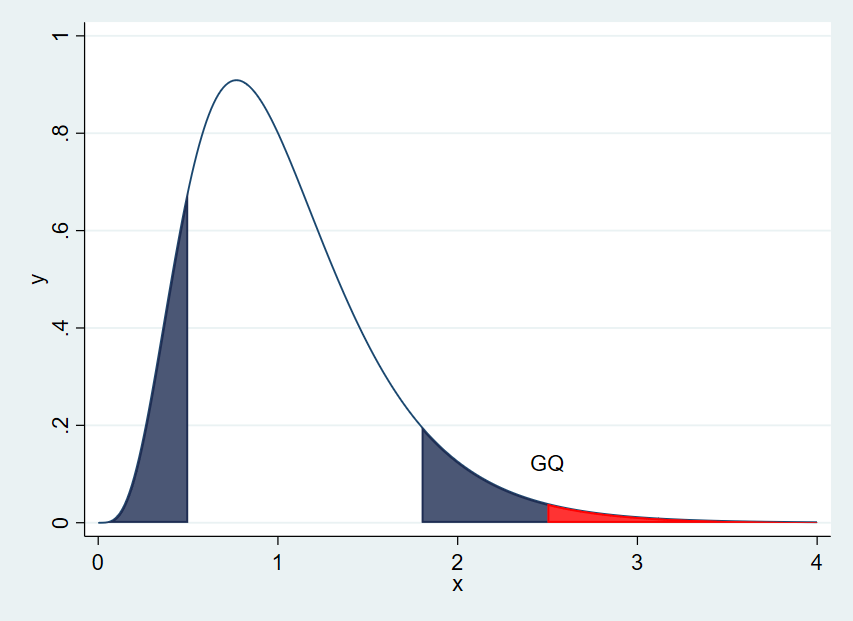
\includegraphics[width=0.8\textwidth]{../Results/F_demo.png}
    \end{figure}
    

\end{frame}

\begin{frame}[fragile]
    \begin{lstlisting}
    
eststo est_c_att0 : reg lnprice bar street school age rich alcohol if attractive == 0
scalar sigma2_0=e(rss)/e(df_r)
scalar df_0 = e(df_r)

eststo est_c_att1 : reg lnprice bar street school age rich alcohol if attractive == 1
scalar sigma2_1=e(rss)/e(df_r)
scalar df_1 = e(df_r)

scalar gq = sigma2_1/sigma2_0
di "GQ      :" gq

di "L Critical value    :" invF(df_1, df_0, 0.025)
di "R Critical value    :" invFtail(df_1, df_0, 0.025)

di "P value  :" Ftail(df_1, df_0, max(gq, 1/gq) )
    \end{lstlisting}

\end{frame}

\begin{frame}[fragile]
    \frametitle{處理異質性變異數 --- 穩健標準誤差}

    穩健標準誤差的好處在於,我們單純從殘差項來調整估計參數的標準誤差,不用考慮這個殘差項跟哪些變數有關係(因此名為穩健)

\begin{lstlisting}
reg lnprice bar street school age rich alcohol attractive, r 
\end{lstlisting}
\vfill
對,就這麼簡單
\end{frame}

\begin{frame}
        \begin{table}
            \centering
            \scalebox{0.7}{
            {
\def\sym#1{\ifmmode^{#1}\else\(^{#1}\)\fi}
\begin{tabular}{l*{2}{c}}
\hline\hline
            &\multicolumn{1}{c}{(1)}&\multicolumn{1}{c}{(2)}\\
            &\multicolumn{1}{c}{OLS}&\multicolumn{1}{c}{OLS with Robust SE}\\
\hline
bar         &       0.216\sym{**} &       0.216\sym{*}  \\
            &    (0.0786)         &    (0.0961)         \\
[1em]
street      &      -0.262\sym{***}&      -0.262\sym{**} \\
            &    (0.0794)         &    (0.0968)         \\
[1em]
school      &       0.164\sym{***}&       0.164\sym{***}\\
            &    (0.0238)         &    (0.0244)         \\
[1em]
age         &     -0.0210\sym{***}&     -0.0210\sym{***}\\
            &   (0.00145)         &   (0.00130)         \\
[1em]
rich        &       0.292\sym{***}&       0.292\sym{***}\\
            &    (0.0304)         &    (0.0296)         \\
[1em]
alcohol     &       0.240\sym{***}&       0.240\sym{***}\\
            &    (0.0358)         &    (0.0377)         \\
[1em]
attractive  &       0.239\sym{***}&       0.239\sym{***}\\
            &    (0.0316)         &    (0.0374)         \\
[1em]
\_cons      &       5.752\sym{***}&       5.752\sym{***}\\
            &    (0.0913)         &     (0.106)         \\
\hline
\(N\)       &        3016         &        3016         \\
\hline\hline
\multicolumn{3}{l}{\footnotesize Standard errors in parentheses}\\
\multicolumn{3}{l}{\footnotesize \sym{*} \(p<0.05\), \sym{**} \(p<0.01\), \sym{***} \(p<0.001\)}\\
\end{tabular}
}

            }
        \end{table}
\end{frame}

\begin{frame}
    \frametitle{處理異質性變異數 --- FGLS}
    假如我們已經知道變異數與哪些因素有關,則可以透過改變資料,或是在回歸中加入權重的方式,來處理異質變異數的問題---廣義最小平方法。

    作法一、土法煉鋼\\
    首先,我們假設變異數跟「年紀」與「美貌」有關
    \begin{enumerate}
        \item 先做一般的OLS
        \item 將殘差的平方取對數 $\ln(u_i^2)$,對「年紀」與「美貌」做回歸
        \item 找出各資料的誤差的估計值,作為修正項 $\hat{h}_i = \exp(\ln(\hat{e}_i^2))$,
        \item 將每一筆資料除上這個修正項,再進行一次回歸
    \end{enumerate}
\end{frame}

\begin{frame}[fragile]

    \begin{lstlisting}
est restore est_a           // 1

predict res_a, residual     // 2
gen ln_res_a2 = ln(res_a^2)
reg ln_res_a2 age attractive

predict ln_e_hat            // 3
gen e_hat=exp(ln_e_hat)

eststo est_FGLS_hand :      /// 4
    reg lnprice bar street school age rich alcohol attractive ///
    [aweight=1/e_hat]\end{lstlisting}

\end{frame}

\begin{frame}[fragile]
    \frametitle{FGLS 內建指令}

    \begin{lstlisting}
eststo est_FGLS :   /// 
    hetregress lnprice bar street school age rich alcohol attractive, /// 
    twostep het(age attractive)
    \end{lstlisting}
    
\vfill
請向 Stata 工程師致敬!回歸人,我的超人 
\end{frame}

\begin{frame}
    \begin{table}
        \centering
        \scalebox{0.6}{
            {
\def\sym#1{\ifmmode^{#1}\else\(^{#1}\)\fi}
\begin{tabular}{l*{5}{c}}
\hline\hline
            &\multicolumn{1}{c}{(1)}&\multicolumn{1}{c}{(2)}&\multicolumn{1}{c}{(3)}&\multicolumn{2}{c}{(4)}                    \\
            &\multicolumn{1}{c}{OLS}&\multicolumn{1}{c}{OLS Robust}&\multicolumn{1}{c}{FGLS by Hand}&\multicolumn{2}{c}{FGLS}                   \\
            &           \_         &           \_         &           \_         &     lnprice         &    lnsigma2         \\
\hline
bar         &       0.216\sym{**} &       0.216\sym{*}  &       0.306\sym{***}&       0.306\sym{***}&                     \\
            &    (0.0786)         &    (0.0961)         &    (0.0779)         &    (0.0779)         &                     \\
[1em]
street      &      -0.262\sym{***}&      -0.262\sym{**} &      -0.172\sym{*}  &      -0.172\sym{*}  &                     \\
            &    (0.0794)         &    (0.0968)         &    (0.0784)         &    (0.0784)         &                     \\
[1em]
school      &       0.164\sym{***}&       0.164\sym{***}&       0.141\sym{***}&       0.141\sym{***}&                     \\
            &    (0.0238)         &    (0.0244)         &    (0.0236)         &    (0.0236)         &                     \\
[1em]
age         &     -0.0210\sym{***}&     -0.0210\sym{***}&     -0.0201\sym{***}&     -0.0201\sym{***}&    -0.00435         \\
            &   (0.00145)         &   (0.00130)         &   (0.00141)         &   (0.00141)         &   (0.00525)         \\
[1em]
rich        &       0.292\sym{***}&       0.292\sym{***}&       0.282\sym{***}&       0.282\sym{***}&                     \\
            &    (0.0304)         &    (0.0296)         &    (0.0296)         &    (0.0296)         &                     \\
[1em]
alcohol     &       0.240\sym{***}&       0.240\sym{***}&       0.265\sym{***}&       0.265\sym{***}&                     \\
            &    (0.0358)         &    (0.0377)         &    (0.0352)         &    (0.0352)         &                     \\
[1em]
attractive  &       0.239\sym{***}&       0.239\sym{***}&       0.240\sym{***}&       0.240\sym{***}&       0.410\sym{***}\\
            &    (0.0316)         &    (0.0374)         &    (0.0364)         &    (0.0364)         &     (0.118)         \\
[1em]
\_cons      &       5.752\sym{***}&       5.752\sym{***}&       5.635\sym{***}&       5.635\sym{***}&      -1.117\sym{***}\\
            &    (0.0913)         &     (0.106)         &    (0.0903)         &    (0.0903)         &     (0.151)         \\
\hline
\(N\)       &        3016         &        3016         &        3016         &        3016         &                     \\
\hline\hline
\multicolumn{6}{l}{\footnotesize Standard errors in parentheses}\\
\multicolumn{6}{l}{\footnotesize \sym{*} \(p<0.05\), \sym{**} \(p<0.01\), \sym{***} \(p<0.001\)}\\
\end{tabular}
}

        }
    \end{table}
\end{frame}

\begin{frame}
    \frametitle{樣本分群}

    剛剛只考慮了樣本分群,誤差變異數不同。但會不會係數也不一樣?

    \begin{itemize}
        \item 兩組樣本誤差是否一樣 --- GQ test
        \item 兩組樣本係數是否一樣 --- Chow test
    \end{itemize}
\end{frame}

\begin{frame}
    \begin{table}
        \centering
        \scalebox{0.7}{
        {
\def\sym#1{\ifmmode^{#1}\else\(^{#1}\)\fi}
\begin{tabular}{l*{2}{c}}
\hline\hline
            &\multicolumn{1}{c}{(1)}&\multicolumn{1}{c}{(2)}\\
            &\multicolumn{1}{c}{Ugly}&\multicolumn{1}{c}{Pretty}\\
\hline
bar         &       0.498\sym{***}&      -0.550\sym{**} \\
            &    (0.0841)         &     (0.197)         \\
[1em]
street      &      0.0242         &      -1.142\sym{***}\\
            &    (0.0842)         &     (0.233)         \\
[1em]
school      &      0.0939\sym{***}&       0.452\sym{***}\\
            &    (0.0248)         &    (0.0667)         \\
[1em]
age         &     -0.0177\sym{***}&     -0.0411\sym{***}\\
            &   (0.00147)         &   (0.00495)         \\
[1em]
rich        &       0.260\sym{***}&       0.610\sym{***}\\
            &    (0.0303)         &     (0.123)         \\
[1em]
alcohol     &       0.322\sym{***}&      -0.103         \\
            &    (0.0366)         &     (0.116)         \\
[1em]
\_cons      &       5.362\sym{***}&       7.143\sym{***}\\
            &    (0.0963)         &     (0.257)         \\
\hline
\(N\)       &        2600         &         416         \\
\hline\hline
\multicolumn{3}{l}{\footnotesize Standard errors in parentheses}\\
\multicolumn{3}{l}{\footnotesize \sym{*} \(p<0.05\), \sym{**} \(p<0.01\), \sym{***} \(p<0.001\)}\\
\end{tabular}
}

        }
    \end{table}
\end{frame}

\begin{frame}[fragile]
    \frametitle{用 Chow test 檢定兩組係數是否相同}

\begin{lstlisting}
eststo est_d : reg lnprice ( i.bar i.street i.school c.age i.rich i.alcohol )##attractive
testparm 1.attractive#1.* 1.attractive#c.*
\end{lstlisting}

其結果為:
\begin{align*}
    F_{7,  3002} =   29.95 \\
    Prob > F =    0.0000
\end{align*}
兩者係數顯著不一樣。


\end{frame}

\begin{frame}
    \frametitle{這是一個可行的 Chow test嗎?}

    \begin{alertblock}{Chow test 的前提}
        Chow test 需要兩個群體的變異數是相同的!而前面已經檢定過,兩者變異數會不同!
    \end{alertblock}

    

\end{frame}